\newcommand{\Q}{\ensuremath{\mathcal{Q}}}
\newcommand{\thetaQ}{\ensuremath{\theta_{\scriptscriptstyle \Q}}}


\begin{figure*}
  \setlength\tabcolsep{2em}
  \begin{tabular}{ll}
    (a) & (b) \\
    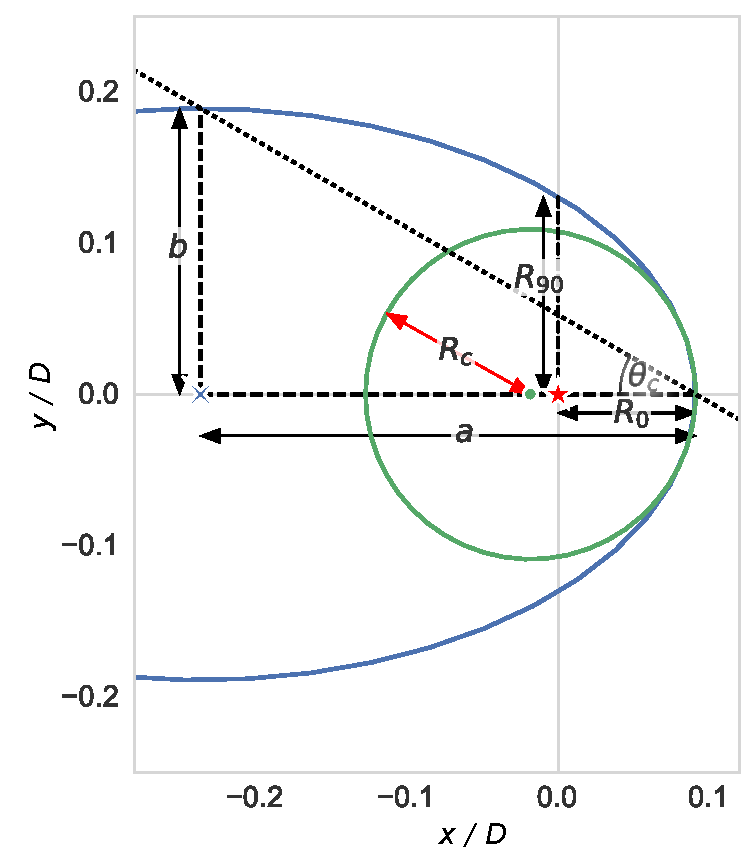
\includegraphics[height=0.45\linewidth]{figs/ellipse_edited}
        & 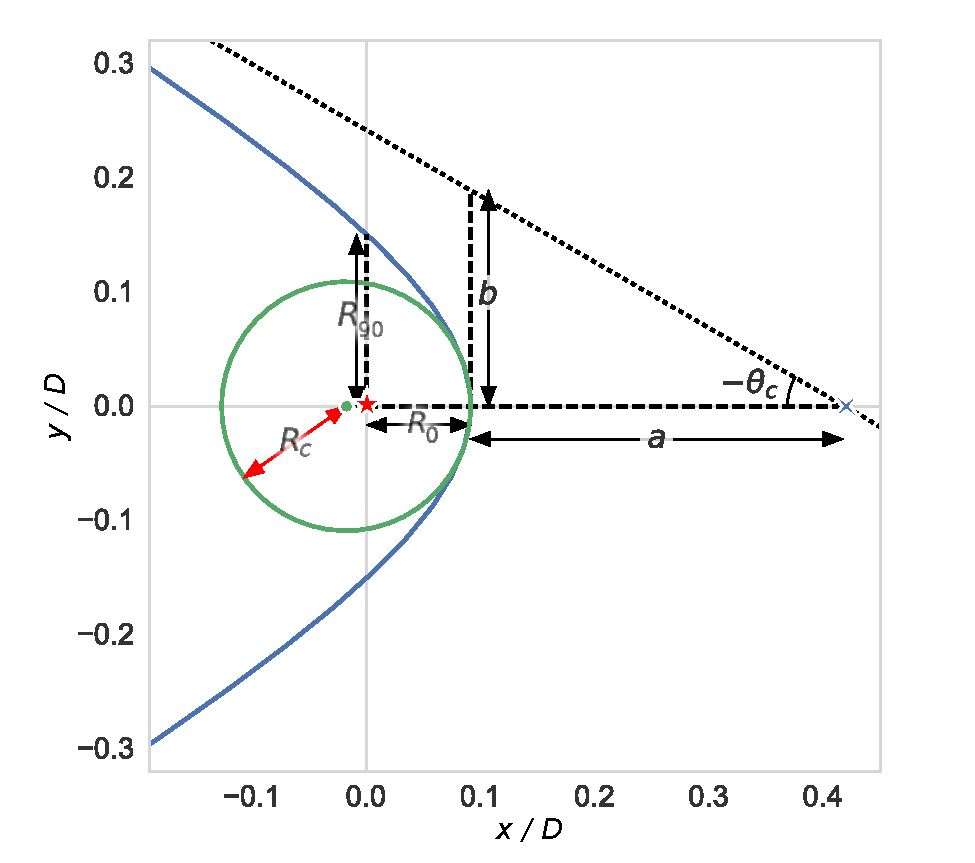
\includegraphics[height=0.45\linewidth]{figs/hyperbola_edited}
  \end{tabular}
  \caption{Example off-center conic sections that can form quadrics of
    revolution: (a) ellipse, (b) hyperbola.  The relationship is shown
    between the conic section parameters \(a\), \(b\), \(\thetaQ\) and the
    bowshock characteristic radii \(R_0\), \(R_{90}\), \(R_c\), as
    defined in Fig.~\ref{fig:characteristic-radii}. The origin (center
    of the weaker flow) is indicated by a red star, the center of
    curvature of the apex of the bow shock is indicated by a green
    dot, and the geometric center of the conic section is indicated by
    a blue cross, which is offset by \(x_0\) from the origin.  Note
    that \(R_0\), \(R_{90}\), \(R_c\), \(a\), and \(b\) are all
    \emph{lengths} and are always positive, whereas \(x_0\) is a
    \emph{displacement} and may be positive or negative.}
  \label{fig:conics}
\end{figure*}
\begin{figure}
  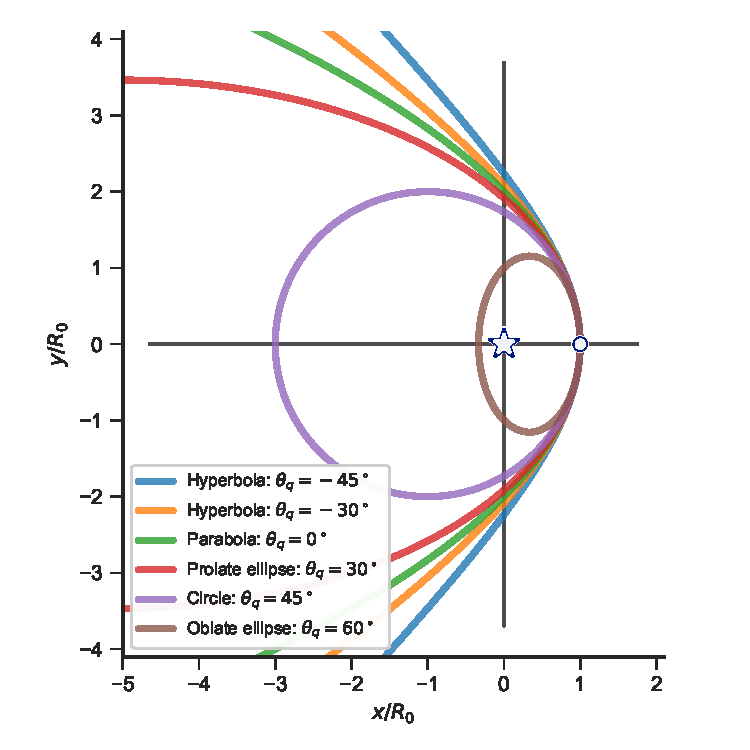
\includegraphics[width=\linewidth]{figs/conic1}
  \caption{Example of a family of conic sections, all with the same
    planitude (flatness at apex, marked by white dot):
    \(\Pi = R_c/R_0 = 2 \). The quadric angle, \(\thetaQ\), varies over
    the family (see text), with lower values of \(\thetaQ\) giving
    larger values of the alatude, \(\Lambda = R_{90}/R_0 \), meaning more
    open wings.  Different values of \(\Pi\) can be achieved for the
    exact same quadrics by sliding them along the \(x\)-axis, which
    will also change the axis scales since these are normalized by
    \(R_0\).}
  \label{fig:conics-family}
\end{figure}


\section{Quadrics of revolution}
\label{sec:conic}


For an arbitrary surface of revolution, application of
equations~(\ref{eq:tanphi}, \ref{eq:tangential}) to determine the
projected shape of the tangent line is not straightforward and in
general requires numerical techniques.  However, analytical results
can be found for the important class of surfaces known as
\textit{quadrics of revolution} \citep{Goldman:1983a, Gfrerrer:2009a},
which are formed by rotating a conic section plane curve about its
symmetry axis.  Examples are the sphere, spheroids (oblate and
prolate), and right circular paraboloids and hyperboloids.\footnote{We
  consider only the case of a single sheet of a 2-sheet hyperboloid or
  paraboloid, since these are the versions that resemble a bow,
  whereas the 1-sheet versions resemble the waist of an hourglass.}
We ignore the degenerate cases of cylinders, cones, and pairs of
parallel planes.  While mathematically simple, these quadrics are
sufficiently flexible that they can provide a useful approximation to
more complex bow shock shapes.

%The 
%In this section we will analyze the case where the resultant shape  of the bow shock is a conic curve (circle, ellipse, parabola or hyperbola).
%These curves are mathematical simple to model and give us a good reference to understand the effects of the projection effects
%described in the last section on other bow shocks. The source of the inner wind is located at the origin, and the center of the conic is located at
%a distance $x_0$ from the source.

%Instead of the excentricity, we utilize the parameter $\theta_c$ to characterize the different curves, where
%$\tan\theta_c = \frac{b}{a}$,  $b$ and $a$ are the typical parameters of conics. A positive value for $\theta_c$ indicates that the given curve is a closed one, i.e
%an ellipse, while a negative value indicates that is an hyperbola. %Insert figures if neccesary  

The shape of the quadric curves in the \(xy\) plane (\(\phi = 0\)) are
shown in Figure~\ref{fig:conics}(a) and (b) for the ellipse and
hyperbola case, respectively.  The conic section itself is fully
described by two lengths, \(a\) and \(b\), which are the
semi-axes.\footnote{Note that we do not require that \(a > b\), so
  either \(a\) or \(b\) may be the semi-major axis.}  However, the
curve can be translated along the \(x\) axis to an arbitrary point
with respect to the star, so that the apex distance \(R_0\) has no
necessary relation to \(a\) or \(b\) and therefore the star/bow
combination requires \emph{three} independent lengths for its
specification.  The displacement \(x_0\) from the star to the
``center'' of the conic section is
\begin{equation}
  \label{eq:conic-x0}
  x_0 = R_0 - \sigma a
  \quad \text{with} \quad
  \sigma = \begin{cases}
    +1 & \text{ellipse}\\
    -1 & \text{hyperbola}
  \end{cases} \ .
\end{equation}
For hyperbolas the center is ``outside'' of the bow and \(x_0\) is
always positive, whereas for ellipses the center is ``inside'' the bow
and \(x_0\) is usually negative, except when \(a < R_0\) (see
Figure~\ref{fig:conics}).

A general parametric form\footnote{%
  The special case of the parabola needs to be treated differently,
  see Appendix~\ref{app:parabola}.} %
for the \(xy\) coordinates of the quadrics (in the \(\phi = 0\) plane,
and with the star at the origin) as a function of \(t = [0, \pi]\) is
then
\begin{gather}
  \label{eq:par-xy}
  \begin{aligned}
    x &= x_0 + \sigma a \Cos(t) \\ 
    y &= b\Sin(t) 
  \end{aligned}
\end{gather}
where
\begin{equation}
  \label{eq:sin-sinh-etc}
  \Sin{}, \Cos = \begin{cases}
    \sin{}, \cos & \text{ellipse}\\
    \sinh{}, \cosh & \text{hyperbola}
  \end{cases}
\end{equation}
Except for the circle case (\(\sigma = +1\), \(a = b\)), the parametric
variable \(t\) is not actually an angle in physical space.  Instead,
the polar form of the bow shape \(R(\theta)\) must be found by substituting
equations~\eqref{eq:par-xy} into \(\theta = \tan^{-1} y/x\) and
\(R = (x^2 + y^2)^{1/2}\).

The type of quadric surface can be characterized by the
\textit{quadric parameter}:
\begin{equation}
  \label{eq:Tq}
  \Q \equiv \sigma \frac{b^2} {a^2} \ , 
\end{equation}
where \(\Q < 0\) corresponds to open surfaces (hyperboloids) and
\(\Q > 0\) corresponds to closed surfaces (oblate spheroids with
\(\Q > 1\) and prolate spheroids with \(\Q < 1\)).  Special cases are
the sphere (\(\Q = 1\)) and the paraboloid (\(\Q = 0\)).
Alternatively, one can define a \textit{quadric angle}:
\(\thetaQ = \sigma \tan^{-1} (b/a)\), which is marked in
Figure~\ref{fig:conics}.  In the case of hyperboloids, the asymptotic
opening angle of the wings (\S~\ref{sec:plan-alat-bow} and
Fig.~\ref{fig:characteristic-radii}) is
\(\theta_\infty = \pi + \thetaQ\) (note that \(\thetaQ < 0\) in this case), and
the minimum slope angle is \(\alpha_{\mathrm{min}} = \abs{\thetaQ}\), see
discussion following equation~\eqref{eq:thetapar}.   

\begin{figure*}
  \centering
  \setkeys{Gin}{width=0.48\linewidth}
  \begin{tabular}{@{}ll@{}}
    (a) & (b) \\
    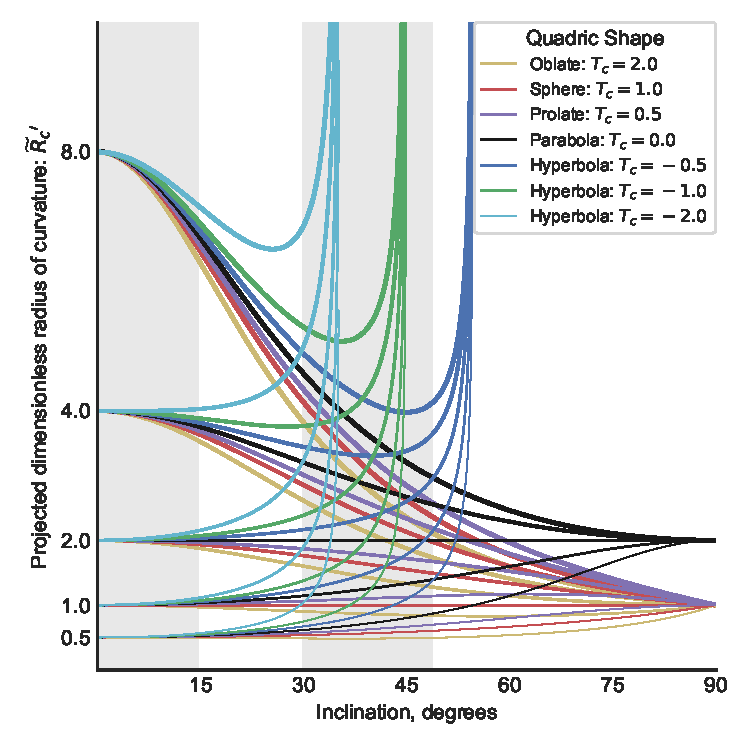
\includegraphics{figs/projected-Rc-vs-i}
        & 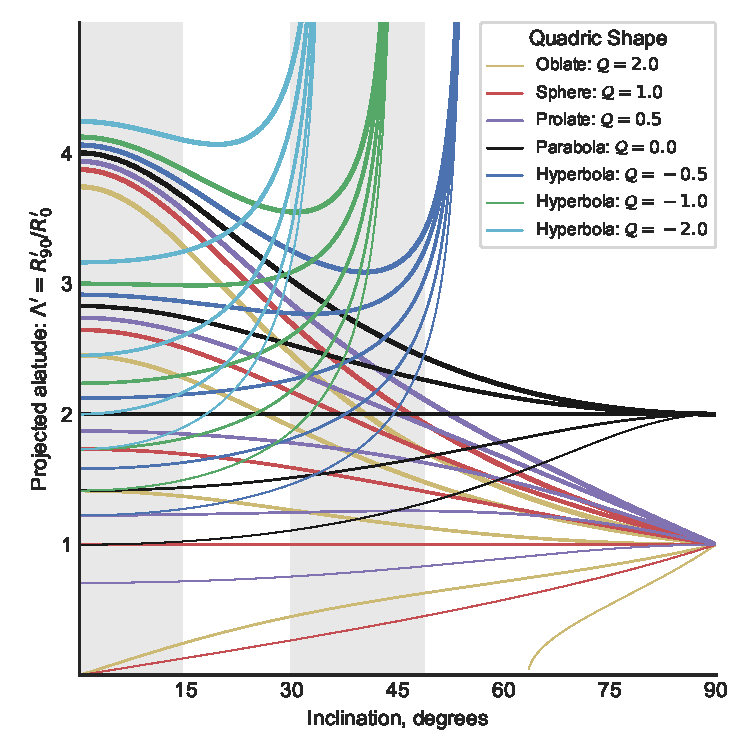
\includegraphics{figs/projected-R90-vs-i}
  \end{tabular}
  \caption[]{Effects of projection on quadrics of revolution:
    variation with inclination, \(\abs{i}\), of bow size and shape.
    Different line colors correspond to varying quadric parameter,
    \(\Q\), (see key), while variation in line width corresponds to
    variation in the ``true'' planitude, \(\Pi\), or apex radius of
    curvature. Vertical gray rectangles show quartiles of
    \(\abs{\sin i}\), which will be equally populated for an isotropic
    distribution of orientations. (a)~Projected planitude:
    \(\Pi'\). (b)~Projected alatude, \(\Lambda'\).}
  \label{fig:quadric-projection}
\end{figure*}

The set of parameters \((\Q, a, x_0)\) are then sufficient to
characterize the star/bow combination, where \(a\) is the quadric
scale and \(x_0\) is its center displacement from the star.  However,
we can also characterize the star/bow by \((R_0, \Pi, \Lambda)\), where
\(R_0\) is the star-apex distance, and \(\Pi\) and \(\Lambda\) are the
planitude and alatude, see \S~\ref{sec:plan-alat-bow}.  We now derive
the equivalences between these two descriptions.  The apex radius of
curvature for a conic section is
\begin{equation}
  \label{eq:Rc-conic}
  R_c = \frac{b^2}{a} = a \abs{\Q}\ ,
\end{equation}
whereas the perpendicular radius, \(R_{90}\), is the value of \(y\)
when \(x = 0\), which can be found from equations (\ref{eq:conic-x0},
\ref{eq:par-xy}) as
\begin{equation}
  \label{eq:conic-R90}
  R_{90}^2 = \Q \left(\sigma a^2 - x_0^2\right) \ .
\end{equation}
Combining equations (\ref{eq:planitude}, \ref{eq:alatude},
\ref{eq:conic-x0}, \ref{eq:Tq}--\ref{eq:conic-R90}) yields
\begin{align}
  \label{eq:R0-from-Q-a-x0}
  R_0 &= x_0 + \sigma a  \\
  \label{eq:Pi-from-Q-a-x0}
  \Pi &= \frac{a \Q}{a + \sigma x_0} \\
  \label{eq:Lambda-from-Q-a-x0}
  \Lambda &= \left( \Q \frac{a - \sigma x_0} {a + \sigma x_0}  \right)^{1/2}
\end{align}
with \(\sigma = \sgn Q\).  It also follows that the quadric parameter in
terms of the planitude and alatude is
\begin{equation}
  \label{eq:Tq-from-Pi-Lambda}
  \Q = 2 \Pi - \Lambda^2 
\end{equation}
% \begin{align}
%   \label{eq:a-from-R0-Pi-Lambda}
%   a &= R_0 \frac{ \Pi  } { \left|  2 \Pi - \Lambda^2\right| } \\
%   x_0 &= R_0 \frac{\Pi - \Lambda^2} {2 \Pi - \Lambda^2}
% \end{align}
Hence, it is the sign of \(2 \Pi - \Lambda^2\) that determines
\(\sigma\) and whether a quadric is a spheroid or a hyperboloid.  For
example, for a constant planitude, \(\Pi\), we can have a family of
different quadric types, with varying alatude, \(\Lambda\), that increases
from oblate, through prolate and paraboloid, to hyperboloid, as
illustrated in Figure~\ref{fig:conics-family}.

% We have set a whole family of curves with a singular parameter denoted as:
% \begin{align}
%   \tan\theta_c \equiv \pm\frac{b}{a}\label{eq:Thc}
% \end{align}
% Positive values of this parameter describe closed curves (i.e. ellipses) and the negative ones describe open curves (i.e. hyperbolas).
% Particular cases are $\theta_c =\frac{\pi}{4}$,
% which describes a circle and $\theta_c=0$, which describes a parabola.
% To determine uniquely a given conic in terms of measurable quantities, we use the set of characteristic radii $(R_0,R_c,R_{90})$ in such way the conic
% parameters $(a,b,\theta_c)$ could be derived from the former. Either way, the radius of curvature can be computed as:

% \begin{align}
% R_c = \frac{b^2}{a} \label{eq:Rc-conic}
% \end{align}

% For the rest of the parameters, the equation for ellipses and hyperbolas are very similar:

% \begin{align}
% R_{90} = \left|\tan\theta_c\right|\left[2aR_0\mp R_0^2\right]^{1/2}\label{eq:conic-R90}
% \end{align}


% Now, we can invert equations (\ref{eq:Rc-conic}) and (\ref{eq:conic-R90}) to estimate the parameters $a$ and $b$.
% %But first is useful to define the quantities $\tilde{R}_c \equiv \frac{R_c}{R_0}$ and $\equiv \frac{\tilde{R}_{90}}{R_0}$ for simplification purposes.
% Hereafter is useful to denote with a tilde quantities which are normalized with $R_0$:


% \begin{align}
%   \tilde{a}\equiv \frac{a}{R_0} &= \pm\frac{\tilde{R}_c}{\left(2\tilde{R}_c-\tilde{R}_{90}^2\right)} \label{eq:a-con}\\
%   \tilde{b}\equiv \frac{b}{R_0} &= \frac{\tilde{R}_c}{\left|2\tilde{R}_c-\tilde{R}_{90}^2\right|^{1/2}} \label{eq:b-con}
% \end{align}


% Dividing equations (\ref{eq:a-con}) and (\ref{eq:b-con}) and substituting into equation (\ref{eq:Thc}) we get:

% \begin{align}
% \tan\theta_c = \pm \left|2\tilde{R}_c-\tilde{R}_{90}^2\right|^{1/2} \label{eq:th_c}
% \end{align}

% Note that the term $2\tilde{R}_c-\tilde{R}_{90}^2$ acts as a discriminant which determine the quadric we are working with.

%The transformation between the conic parameters and the characteristic radii are given by:
%\begin{align}
%R_c &= \frac{b^2}{a} \\
%R_{90} &= b\left[\pm\left(1 - \frac{(a \mp R_0)^2}{a^2}\right)\right]^{1/2}\label{eq:r90-conic}
%\end{align}ut 
%In (\ref{eq:r90-conic}), the positive sign correspond to an elliptic quadric, while the negative sign to an hyperbolic quadric.
%The inverse transformation of (\ref{eq:Rc-conic}) and (\ref{eq:r90-conic}) is given by:
%\begin{align}
%\frac{a}{R_0} &= \frac{A}{2A-B^2} \label{eq:a-conic}\\
%\frac{|b|}{R_0} &= \frac{A}{\left|2A-B^2\right|^{1/2}}\\
%\tan\theta_c &= \frac{2A-B^2}{\left|B^2 - 2A\right|^{1/2}} \label{eq:thc-conic} \\
%\mathrm{where:~} B &\equiv \frac{R_{90}}{R_0} \\
%#A &\equiv \frac{R_c}{R_0}
%\end{align}

\subsection{Plane-of-sky projection of quadric surfaces} 

We now apply the machinery of \S~\ref{sec:projection} to find the
projected shape of a quadric bow on the plane of the sky.  The
intrinsic 3D shape of the shell is given by rotating
equations~\eqref{eq:par-xy} about the \(x\)-axis, but it is more
convenient to first transform to a reference frame where the origin is
at the center of the conic section:
\begin{equation}
  \label{eq:xyz-XYZ}
  (X, Y, Z) = (x - x_0, y, z) . 
\end{equation}
In this new frame, the quadric shape is
\begin{gather}
  \label{eq:quadric-XYZ}
  \begin{aligned}
    X &= a\Cos(t) \\ 
    Y &= b \Sin(t)\cos\phi \\
    Z &= b \Sin(t)\sin\phi
  \end{aligned}
\end{gather}
The azimuth of the tangent line as a function of inclination and
parametric variable is then found from equations (\ref{eq:alpha},
\ref{eq:tanphi}) to be
\begin{equation}
  \label{eq:phit-quadric}
  \sin\phi_{\T} = \frac{b \Cos(t)} {a \Sin(t)} \tan i \ .
\end{equation}
Combining equations~(\ref{eq:Trans}, \ref{eq:quadric-XYZ},
\ref{eq:phit-quadric}) gives the observer-frame cartesian
plane-of-sky coordinates of the tangent line:
\begin{gather}
  \label{eq:conic-projected-XY}
  \begin{aligned}
    X_{\T}' & = \frac{\Cos(t)}{a\cos i}
    \left(a^2\cos^2 i + \sigma b^2\sin^2 i\right)
    \\
    Y_{\T}' &= b\Sin(t)
    \left(
      1 - \frac{b^2 \Cos^2(t)}{a^2 \Sin^2(t)}
      \tan^2 i\right)^{1/2}
  \end{aligned}
\end{gather}
We wish to show that this projected shape is a conic section of the
same variety (ellipse or hyperbola) as the one that generated the
original quadric.  If this \emph{were} true, then it would be possible
to write the plane-of-sky coordinates as
\begin{gather}
  \begin{aligned}
    X_{\T}' &= a'\Cos( t')  \\
    Y_{\T}' &= b'\Sin (t')  . 
  \end{aligned}\label{eq:conic-projected-XY-conic}
\end{gather}
Comparing equations (\ref{eq:conic-projected-XY}) and
(\ref{eq:conic-projected-XY-conic}), we find after some algebra that
the two forms for \((X_{\T}', Y_{\T}')\) are indeed consistent, with
the equivalences:
%
\newcommand\fQi{\ensuremath{f_{\scriptscriptstyle \Q,i}}}
\begin{align}
  \label{eq:a-prime}
  a' &= a \fQi \cos i  \\
  \label{eq:b-prime}
  b' &= b \\
  t' &= \Cos^{-1} \left[ \fQi \Cos(t) \right]  \ ,
  % t' &= \Cos^{-1} \left[  \frac{a'\Cos(t)}{a\cos i}\right] \ .
\end{align}
where for convenience we define the quadric projection factor:
\begin{equation}
  \label{eq:fQi-factor}
  \fQi = \left( 1 + \Q \tan^2 i \right)^{1/2} \ .
\end{equation}
This demonstrates the original claim that the projected shape is also
a conic section, which means that we can re-use the previous
equations~(\ref{eq:R0-from-Q-a-x0}--\ref{eq:Tq-from-Pi-Lambda}) with
primed quantities substituted for unprimed ones.  From
equations~(\ref{eq:Tq}, \ref{eq:a-prime}, \ref{eq:b-prime}) it follows
that the quadric parameter of the projected shape is
\begin{equation}
  \label{eq:Q-prime}
  \Q' = \frac{ \Q } { \fQi^2 \cos^2 i} \ .
\end{equation}
Finally, we transform the projected reference frame back to be
centered on the star again:
\begin{equation}
  \label{eq:XYZ-xyz-prime}
  (x_{\T}', y_{\T}') = (X_{\T}' + x_0', Y_{\T}') \ , 
\end{equation}
where the projected quadric displacement \(x_0'\) follows from simple
foreshortening:
\begin{equation}
  \label{eq:x0-prime}
  x_0' = x_0 \cos i \ .
\end{equation}

\begin{figure*}
  \centering
  \setkeys{Gin}{width=0.48\linewidth}
  \begin{tabular}{@{}ll@{}}
    (a) & (b) \\
    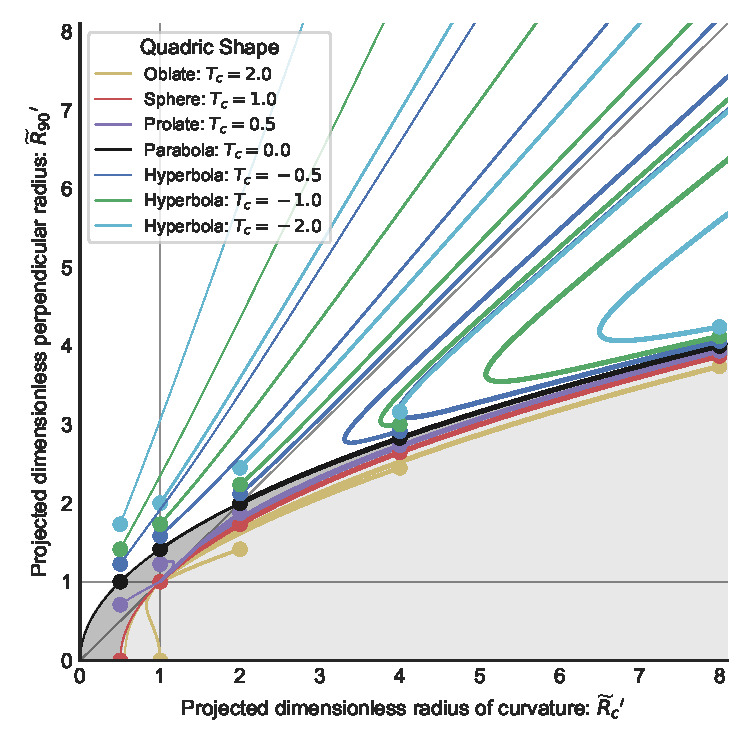
\includegraphics{figs/projected-R90-vs-Rc}
    & 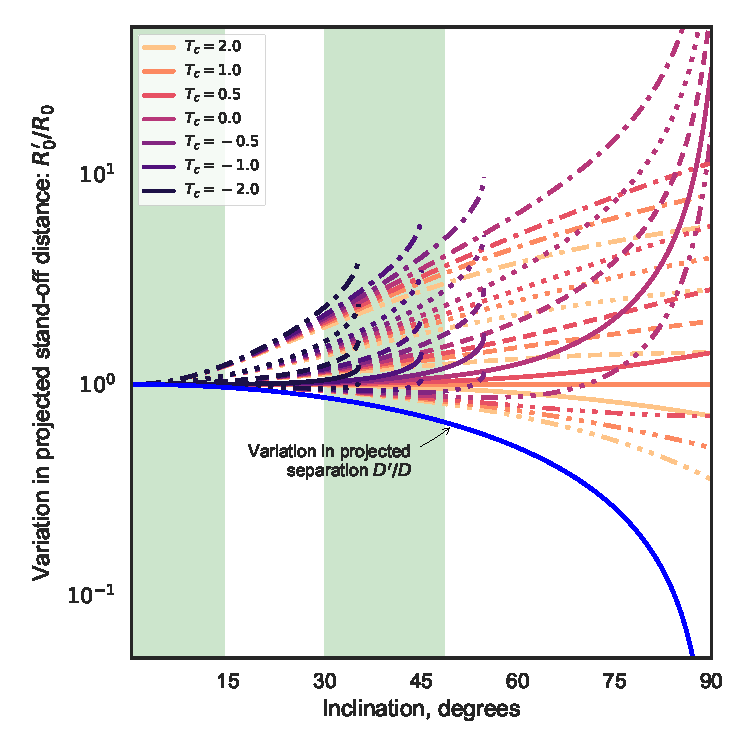
\includegraphics{figs/projected-R0-vs-i}
  \end{tabular}
  \caption[]{ As Figure~\ref{fig:quadric-projection}, but %
    (a)~diagnostic planitude--alatude diagram: \(\Lambda'\) versus
    \(\Pi'\), and %
    (b)~projected/true star-apex distance: \(R_0' / R_0\) versus
    \(\abs{i}\). %
    In (a), shading indicates different classes of quadrics:
    hyperboloids (white), prolate spheroids (dark gray), and oblate
    spheroids (light gray), with the limiting case of paraboloids
    shown by the thin black line.}
  \label{fig:quadric-projection-continued}
\end{figure*}

\begin{figure*}
  \centering
  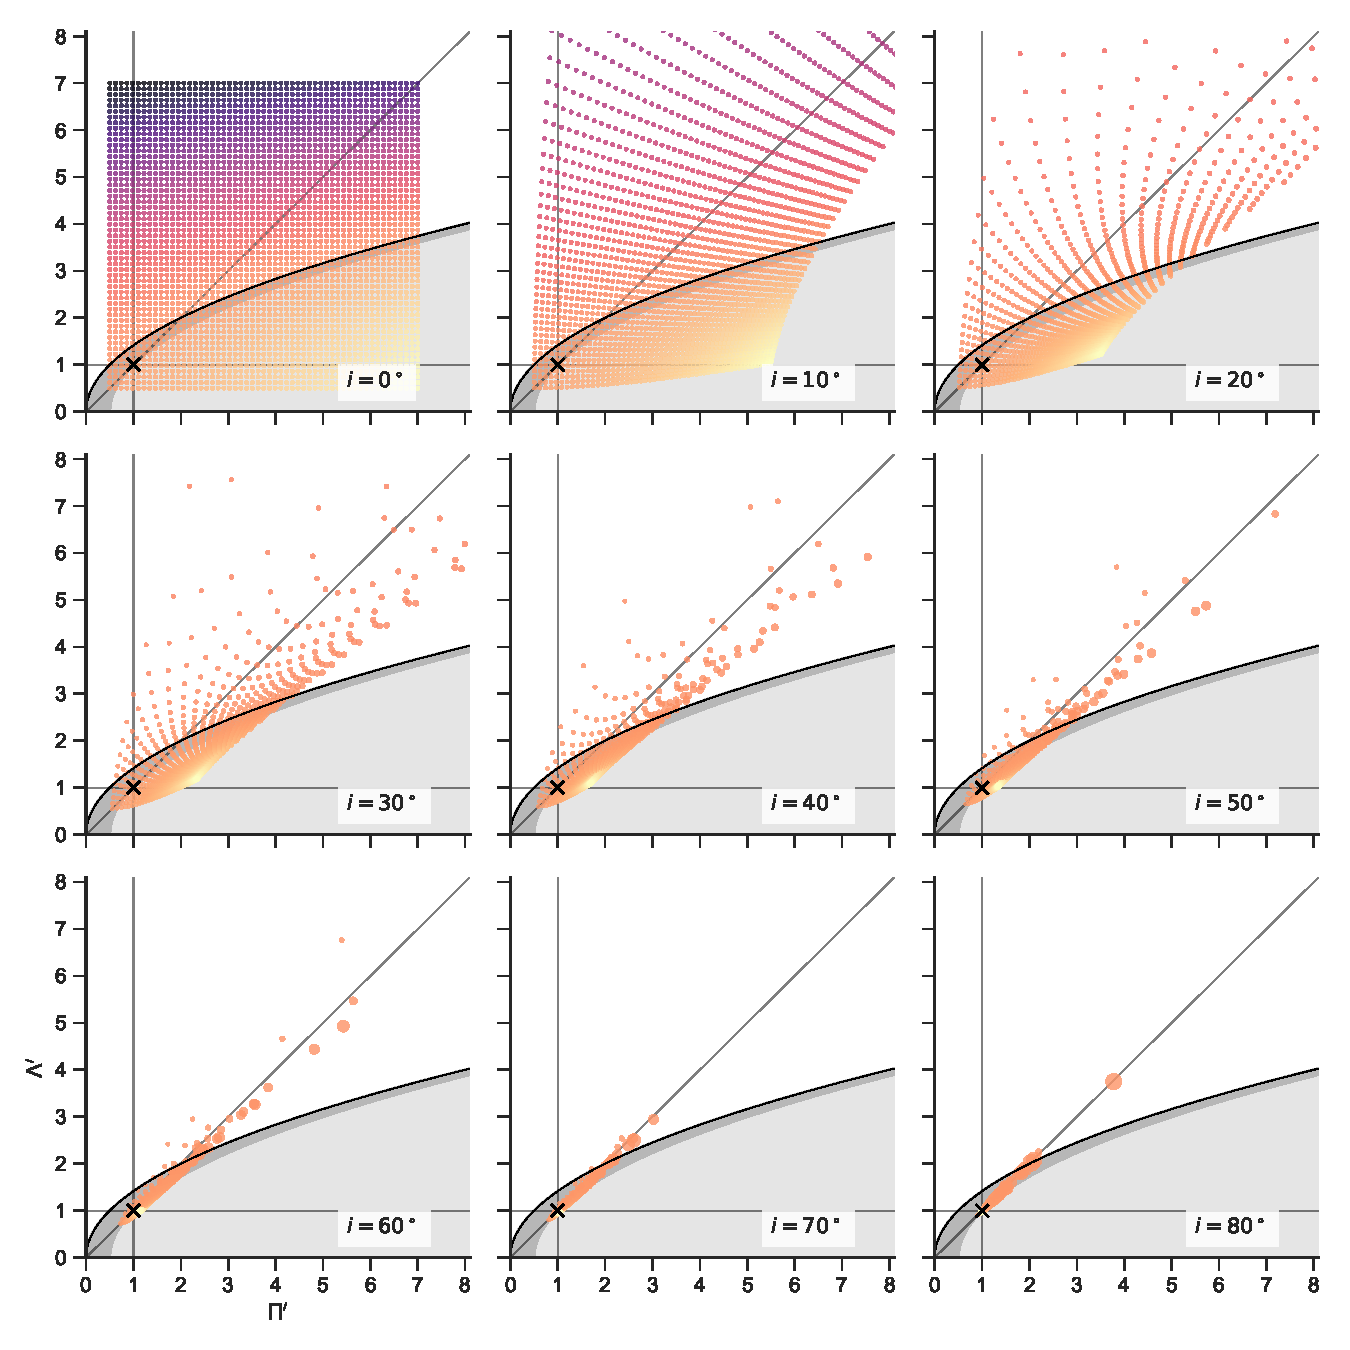
\includegraphics[width=\linewidth]{figs/projected-R90-Rc-snapshots}
  \caption{Variation with inclination angle of the apparent shape of
    quadric bows with true planitude and alatude that are uniformly
    distributed over the ranges \(\Pi = [0.5, 4.5]\),
    \(\Lambda = [0.5, 4.5]\).  Panels show the apparent
    \((\Pi', \Lambda')\) as the inclination is increased through uniform
    intervals in \(\abs{sin i}\).  Symbol color represents the quadric
    parameter, \(\Q\), increasing from dark blue, through orange, to
    yellow. Symbol size is proportional to the increase in apparent
    star--apex distance, \(R_0'/R_0\).}
  \label{fig:projected-R90-Rc-snapshots}
\end{figure*}

The projection of the apex distance then follows from the primed
version of equation~\eqref{eq:R0-from-Q-a-x0} as
\begin{equation}
  \label{eq:R0-prime}
  \frac{R_0'}{R_0} =
  \cos i \left[ 1 + \frac{\Pi} {\Q} \bigl(\fQi - 1\bigr) \right]
\end{equation}
and the projected planitude and alatude can be calculated from
equations~(\ref{eq:Pi-from-Q-a-x0}, \ref{eq:Tq-from-Pi-Lambda},
\ref{eq:a-prime}, \ref{eq:Q-prime}) as
\begin{align}
  \label{eq:Pi-prime}
  \Pi' &= \frac{\Pi}{(R_0'/R_0)\, \fQi \cos i } \\
  \label{eq:Lambda-prime}
  \Lambda' &= \left( 2 \Pi' - \Q' \right)^{1/2} \ .
\end{align}
These are all shown in Figures~\ref{fig:quadric-projection}
and~\ref{fig:quadric-projection-continued} for a variety of quadric
parameter \(Q\) (line color) and true planitude \(\Pi\) (line
thickness).  The projected planitude and alatude
(Fig.~\ref{fig:quadric-projection}) behave in a qualitatively similar
fashion.  Whatever the true values of \(\Pi\) and \(\Lambda\), all spheroids
(\(\Q > 0\)) tend towards \(\Pi' = 1\) and \(\Lambda' = 1\) as the inclination
increases towards \(90^\circ\).  This is because when the spheroid is
oriented edge-on, we see its circular cross-section.  Hyperboloids
behave differently: although \(\Pi'\) and \(\Lambda'\) initially decrease with
increasing inclination (for true \(\Pi > 2\)), they turn around and
increases again as \(\abs{i}\) approaches the critical value
\(i_{\mathrm{crit}} = 90^\circ - \abs{\thetaQ}\).  For
\(\abs{i} > i_{\mathrm{crit}}\) the tangent line does not exist (see
\S~\ref{sec:tangent-line}) because the line of sight is ``inside'' the
asymptotic cone of the far wings (with opening half angle
\(\alpha_{\mathrm{min}} = \abs{\thetaQ}\)), and so no limb-brightened shell
would be visible.\footnote{%
  As illustrated in Figure~8 of \citet{Graham:2002a}, the isophotal
  emission contours are elliptical in such a case (assuming
  cylindrical symmetry) and no curved bow shape is apparent.
  Deviations from cylindrical symmetry \emph{can} result in a curved
  emission arc, even for this no-tangent case
  (\citeauthor{Graham:2002a}'s Fig.~9), but that is beyond the scope
  of this paper.} For paraboloids and spheroids,
\(\alpha_{\mathrm{min}} = 0\), which means that the tangent line exists for
all viewing angles.

In Figure~\ref{fig:quadric-projection-continued}a, we show the
inclination-dependent tracks of the quadrics in the diagnostic
\(\Pi'\)--\(\Lambda'\) plane of projected alatude versus projected planitude.
The true planitude and alatude, which are seen for an edge-on viewing
angle \(i = 0^\circ\), are marked by filled circles.  The zones
corresponding to each class of quadric (oblate spheroid, prolate
spheroid, or hyperboloid) are marked by gray shading, and it can be
seen that the tracks never cross from one zone to another. The
convergence of all the spheroid tracks on the point
\((\Pi', \Lambda') = (1, 1)\) is apparent, as is the divergence of the
hyperboloid tracks towards \((\Pi', \Lambda') = (+\infty, +\infty)\).  The paraboloids,
by contrast, converge on the point \((\Pi', \Lambda') = (2, 2)\), and the
special case of the confocal paraboloid,\footnote{So named because the
  star is at the focus of the parabola.} with true planitude and
alatude \((\Pi, \Lambda) = (2, 2)\), is the only quadric whose apparent shape
remains identical for all inclination angles.  

Figure~\ref{fig:quadric-projection-continued}b shows how the apparent
star-apex separation varies with inclination.  For moderate
inclinations, \(\abs{i} < 30^\circ\), this depends primarily on the true
planitude \(\Pi\), with very little influence of the quadric parameter
\(\Q\).  For \(\Pi > 1\), the separation increases with \(\abs{i}\), whereas
for \(\Pi < 1\) it decreases slightly.  Note, however, that for cases
where the projected distance to the source of the external flow,
\(D'\), can be measured, then \(R_0'/D'\) is always an increasing
function of \(\abs{i}\).  For larger inclinations, \(\abs{i} > 30^\circ\), the
strands for different \(\Q\) begin to separate, with hyperbolae
showing the strongest increase of \(R_0'\) with \(\abs{i}\).

A complementary view of the effects of projection is shown in
Figure~\ref{fig:projected-R90-Rc-snapshots}, which shows ``snapshots''
of \((\Pi', \Lambda')\) for a sequence of 6 values of the inclination, equally
spaced in \(\abs{\sin {i}}\), so that each panel is equally likely for
an isotropic distribution of orientations.  The distribution of the
true \(\Pi\) and \(\Lambda\) are each assumed to be uniform on the range
\([0.5, 4.5]\), giving a uniformly filled square of values for
\(\abs{i} = 0\), which becomes increasingly distorted as \(\abs{i}\)
increases.  The color scale represents \(\Q\) and the symbol size is
proportional to \(R_0'/R_0\).  It can be seen that the points tend to
cluster closer and closer to the diagonal, \(\Lambda' = \Pi'\), as the
inclination increases, and that the points just below this line tend
to have the largest values of \(R_0'/R_0\).  The green shaded region
shows the zone of true \(\Lambda, \Pi\) for hyperboloids where the tangent
lines still exists for that value of \(\abs{i}\).  This becomes
smaller and smaller as \(\abs{i}\) increases, which explains why the
hyperboloid zone becomes increasingly depopulated: all quadrics that
lay above this region when \(i = 0^\circ\) will no longer be visible as a
bow for this value of \(\abs{i}\).  Note that this figure is merely
illustrative of the qualitative effects of projection, since in
reality there is no particular reason to expect a uniform distribution
in true \(\Pi\) and \(\Lambda\).

% Finally, using $D' = D\cos i$ and substituting $a'$ instead of $a$ in equation (\ref{eq:x0}) we find that: 

% \begin{align}
% R'_0 &= \pm a' + x_0\cos i \\
% R'_0 &= \pm\left(a^2\cos^2 i \pm b^2\sin^2 i\right)^{1/2} +  (R_0 \mp a)\cos i
% \end{align}

% Defining  $f(i;\theta_c)\equiv\left(1\pm\tan^2\theta_c\tan^2i\right)^{1/2}$ we find that:
% \begin{align}
% \frac{R'_0}{D'}=\frac{R_0}{D}\left(1\pm \tilde{R}_c\cot^2\theta_c(f(i;\theta_c)-1) \right)
% \label{eq:qprime}
% \end{align}
% %Where $A\equiv \frac{R_c}{R_0}$
% The Radius of curvature in the observer's frame is given by $R'_c=\frac{b'^2}{a'}$. Then:
% \begin{align}
%   \tilde{R}_c'\equiv  \frac{R'_c}{R'_0} &= \frac{\tilde{R}_c}{\cos^2 i f(i;\theta_c)\frac{q'}{q}}
%   \label{eq:Aprime}\\
%   \tan\theta'_c & = \frac{\tan\theta_c}{\cos i f(i;\theta_c)} \\
%   \tilde{R}'_{90} &= \left(\frac{2\tilde{R}_cf(i;\theta_c) \mp \tan^2\theta_c\frac{q'}{q}}{\frac{q'}{q}}\right)^{1/2}\frac{\sec i}{f(i;\theta_c)}
% \end{align}
% where $q=\frac{R_0}{D}$ and $q' = \frac{R'_0}{D'}$.

% When $R'_{90}$ is measurable, diagnostic diagrams like figure (\ref{fig:projected-R90-vs-Rc}) can be used to compare with observations.  



 
%%% Local Variables:
%%% mode: latex
%%% TeX-master: "quadrics-bowshock"
%%% End:

